\subsubsubsubsection{Lane sign decorator}
\begin{figure}[h]
\centering
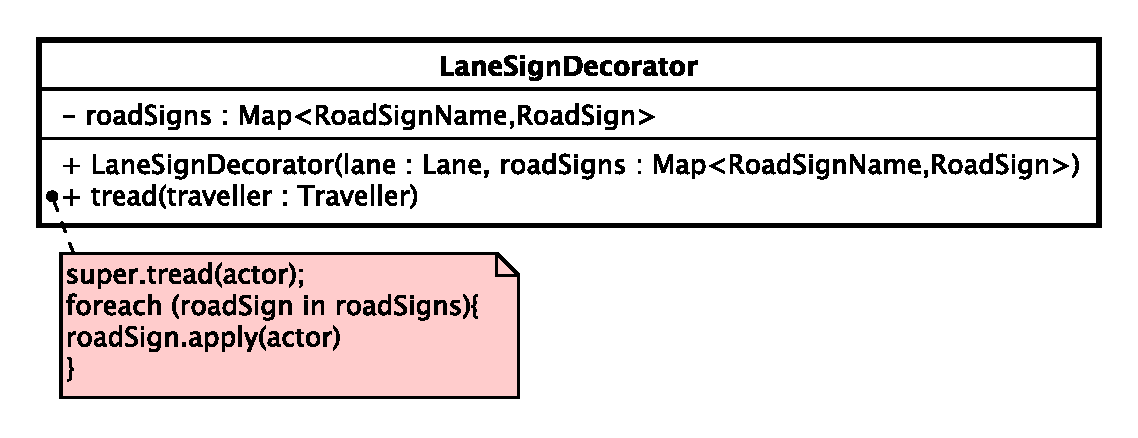
\includegraphics[scale=0.6,keepaspectratio]{images/solution/app/backend/lane_sign_decorator.eps}
\caption{\pReactiveComponentLaneDecoration::LaneSignDecorator}
\label{fig:sd-app-lane_sign_decorator}
\end{figure}
\FloatBarrier
\begin{itemize}
  \item \textbf{\descr} \\
    It represents a decorator which add road signs behaviour on the top of a standard lane behaviour. 
  \item \textbf{\attrs}
  \begin{itemize}
    \item \texttt{roadSigns: Map<RoadSignName, RoadSign>} \\
The map of road signs to consider during the decoration.
  \end{itemize}
  \item \textbf{\ops}
   \begin{itemize} 
   \item[+] \texttt{LaneSignDecorator(lane: Lane, roadSigns: Map<RoadSignName, RoadSign>)} \\
Creates a lane sign decorator with a specific lane to decorate and a map of road signs to apply as decorations.
    \item[+] \texttt{tread(entity: MovingEntity)} \\
Decorates the standard behaviour of the lane with road signs.  
  \end{itemize}
\end{itemize}
